%---------------------------------------------------------%
%______//------             GAC             ------\\______%
%______||------         Chapitre 6          ------||______%
%______\\------  Transformations de Tietze  ------//______%
%---------------------------------------------------------%

\chapter{Transformations de Tietze}
  
  \begin{defi}
  Soit $\langle X_1 , \ldots, X_n | \underbrace{r_1, \ldots, r_m}_{R}\rangle$ une présentation finie d'un
  groupe $G$. Les transformations suivantes, appelées \emph{transformation de Tietze} \index{Transformation de
    Tietze}, changent la présentation sans changer le groupe.
  \end{defi}



   %Algorithme 
   \begin{algorithm}
     \caption{Première transformation de Tietze}
     \label{alg:trans-tietze-1}
     \begin{algorithmic}
       \State $T_1$ ou $R^+$: Ajouter à la présentation de $G$ un relateur $r_{m+1}$ qui appartient à la
       clotûre normale de $R$ (notée $\overline{R}$, $\lhd R \rhd$ ou $gp_G(R)$).
       \State Soit $r_{m+1} \in \overline{R} \setminus R$: $\langle X | R \rangle \xrightarrow{R^+, T_1}
       \langle X | R \cup \{r_{m+1}\} \rangle$.
     \end{algorithmic}
   \end{algorithm}


   \begin{ex}
     Considérons $\Z^2 = \langle a, b | aba^{-1}b^{-1} \rangle \xrightarrow{R^+} \langle a, b | [a,b], [a,b]^2
     \rangle$.
   \end{ex}


   \begin{algorithm}
     \caption{Deuxième transformation de Tietze}
     \label{alg:trans-tietze-2}
     \begin{algorithmic}
       \State $R^-$: Opération inverse de $R^+$.
       \State Soit $r \in R \setminus \overline{R \setminus \{r\}}$. Alors $\langle X | R \rangle
       \xrightarrow{R^-} \langle X | R \setminus \{r\} \rangle$.
     \end{algorithmic}
   \end{algorithm}


   \begin{algorithm}
     \caption{Troisième transformation de Tietze}
     \label{alg:trans-tietze-3}
     \begin{algorithmic}
       \State $X^+$: Ajouter à la présentation de $G$ un générateur $x_{n+1}$ ainsi qu'une relation $x_{n+1} = w(x_1,
       \ldots, x_n)$ (un mot sur $x_1, \ldots, x_n$).
       \State $\langle X | R \rangle \xrightarrow{X^+} \langle X, x_{n+1} | R \cup \{ x_{n+1}w^{-1}(x_1, \ldots, x_n)\} \rangle$
     \end{algorithmic}
   \end{algorithm}


   \begin{algorithm}
     \caption{Quatrième transformation de Tietze}
     \label{alg:trans-tietze-4}
     \begin{algorithmic}
       \State $X^-$: Opération inverse de $X^+$.
       \State Soit $y \in X$, $w \in \langle X \setminus \{y\} \rangle$ et $y^{-1}w$ est le seul mot dans $R$
       qui contient $y$. Alors
       \State $\langle X | R \rangle \xrightarrow{X^-} \langle X \setminus \{y\} | R \setminus \{y^{-1}w\} \rangle$.
     \end{algorithmic}
   \end{algorithm}

   \begin{ex}
     Soit $G = \langle x,y | xyx = yxy \rangle$. C'est le groupe fondamental du noeud de trèfle. On va
     utiliser les transformations de Tietze. On a
     \begin{align*}
       \langle x,y | xyx = yxy \rangle &\xrightarrow{X^+} \langle x,y,a,b | xyx = yxy, a=xy, b=xyx \rangle\\
       &\xrightarrow{R^+} \langle x,y,a,b | xyx=yxy, a=xy, b=xyx, x=a^{-1}b, y = b^{-1} b^{-1}a^2, a^3 = b^2
         \rangle & a^3 = xyxyxy\\
       &\xrightarrow{R^-} \langle x,y,a,b | a^3 = b^2, x = a^{-1}b, y = b^{-1}a^2 \rangle\\
       &\xrightarrow{X^-} \langle a,b | a^3 = b^2 \rangle.
     \end{align*}
     Cette dernière présentation correspond au produit libre amalgamé.
   \end{ex}


   \begin{prop}[de \textsc{Tietze}] \label{prop:de-Tietze} \index{Proposition!de \textsc{Tietze}}
     Les transformations de Tietze ne changent pas le groupe.
   \end{prop}

   \begin{preuve}[pour $X^+$]
     Supposons que $G = \langle X | R \rangle$, $y$ est un symbole qui n'est pas dans $X$, et $w(X)$ un mot
     réduit de $\F(X)$. On veut montrer que $\langle X, y | R \cup \{y^{-1}w(X)\} \rangle \cong \langle X, R
     \rangle = G$. 

     Soit $\phi : \F(X) \to G$ l'homomorphisme donné par la propriété universelle des groupes libres. Le
     groupe libre $\F(X, y)$ sur $X \cup \{y\}$ est engendré librement par $X \cup
     \{y^{-1}w(X)\}$. C'est-à-dire que $\F(X \cup \{y\}) = \F(X \cup \{y^{-1}w(X)\})$. C'est vrai car à
     partir de $y^{-1}w(X)$, on peut obtenir $y$ (cette inclusion est sensée être facile), et à partir de
     $y$ on peut obtenir $y^{-1}w(X)$. Ainsi on a
       \[X \cup \{y^{-1}w(x)\} \hookrightarrow \F(x,y) = \F(X \cup \{y^{-1}w(X)\}.\]
     Il y a un unique homomorphisme $\phi^1: \F(x,y) \to G$ tel que $\phi^1(x) = \phi(x)$ et
     $\phi^1(y^{-1}w(X)) = 1$ pour $x \in X$.

     \begin{center}
       \begin{tikzcd}
         X \cup \{y^{-1} \omega(X)\} \arrow[r] \arrow[d, "f"] & \F(X,y) = \F(X \cup \{y^{-1}\omega(X)\})
         \arrow[d, "\chi"]\\
         G \arrow[ru, leftarrow, "\phi^1!"] \arrow[r, leftarrow, "\phi"] & \F(X)
       \end{tikzcd}
     \end{center}

     ($f(x) = x$ si $x \in X$ et $1$ si $x = y^{-1} \omega(X)$). L'homomorphisme $\phi^1: \F(X,y) \to G$ se factorise comme $F(X,y) \xrightarrow{\chi} \F(X)
     \xrightarrow{\phi} G$ où $\chi(x) = x$ pour tout $x \in X$ et $\chi(y) = w(x)$. Alors $\phi^1$ est
     surjective et
       \[\ker \phi^1 = \chi^{-1}(\phi^{-1}(1)) = \chi^{-1} \left( gp_{\F(X)}R \right) = gp_{\F(X,y)}(R \cup
       \{y^{-1}w(X)\}).\]
     Ainsi par le premier théorème d'isomorphisme, on a que 
       \[G \cong \F(x,y)/\ker \phi^1 = \langle X,y | R \cup \{y^{-1}w(X)\} \rangle.\]
   \end{preuve}



   \begin{theo}[de \textsc{Tietze}] \label{thm:de-Tietze} \index{Théorème!de \textsc{Tietze}}
     Soient ${\cal P}_1 = \langle X | R \rangle$ et $ {\cal P}_2 = \langle Y | S \rangle$ des présentations
     finies pour un groupe $G$. Alors il existe une suite finie de transformations de Tietze qui transforment
     ${\cal P}_1$ en ${\cal P}_2$.
   \end{theo}

   \begin{preuve}
     cf. feuille annexe. $G$ est donné par ${\cal P}_1$ et ${\cal P}_2$. Alors chaque $x \in X$ peut être
     écrit comme un mot sur $Y$, et on note $x(Y)$. Alors $X(Y)$ représente tous les mots sur $Y$ qui
     décrivent les éléments de $X$. De la même manière, on définit $y(X)$ et $Y(X)$. 

     On commence avec ${\cal P}_1$ et on utilise les transformations suivantes (voir feuille annexe).

     Intuitivement, on ajoute tous les générateurs $Y$ et on enlève tous les générateurs $X$. On utilise les
     transformations $R^+$ $|X|+|R|+|Y|+|S|$ fois et $R^- 2(|R|+|Y|)$ fois. Donc il y a un nombre fini de transformations de ${\cal
       P}_1$ à ${\cal P}_2$.
   \end{preuve}

   \begin{cor}
     On peut énumérer toutes les présentations finies d'un groupe $G$ à partir d'une présentation quelconque
     pour $G$.
   \end{cor}

   \begin{prop}
     Si le groupe $G$ a une présentation finie $\langle X_1 |R \rangle$ et une présentation infinie $\langle
     X_2 | S \rangle$ où $S$ est infini, alors il existe un entier $n$ tel que $\langle X_2 | s_1, \ldots, s_n
     \rangle$ est une présentation finie pour $G$.
   \end{prop}

   \section{Algorithme de Todd-Coxeter (1936) (Coset enumeration)}
   \label{sec:algorithme-de-todd-loxeter}

   Étant donné un groupe $G$, défini par une présentation finie $G = \langle X, R \rangle$, et un sous-groupe
   $H$ de $G$ d'indice fini dans $G$, on souhaite énumérer les éléments du quotient $G/H$ et décrire l'action
   de $G$ sur $G/H$. 

   \subsection{Version basique}
   \label{sec:version-basique-todd-coxeter}

      Si $H = \{1\}$, l'algorithme va énumérer les éléments de $G$, si $G$ est fini.

     \begin{algorithm}
       \caption{Algorithme de Todd-Coxeter (basique)}
       \label{alg:todd-coxeter-basique}
       \begin{algorithmic}
         \State $\forall r \in R$, créer un tableau de $|r|+1$ colonnes.
         \State Si $r = x_1 \cdots x_n$, le tableau est
         \State
         \begin{tabular}{c p{2cm} c}
           \begin{tabular}{|ccccccccccc|}
             \hline
             & $x_1$ & & $x_2$ & & $\cdots$ & & $x_1^{-1}$ & & $x_n$ & \\
             \hline
             1 & - & 2 &  & & $\cdots$ & 2 & & 1 & & 1 \\
             2 &  & & & & & & & & & 2\\
             \hline
           \end{tabular}
             & &
                 \begin{tabular}{|c|c|}
                   \hline
                   Définition & Bonus \\
                   \hline
                   $1x_1 = 2$ & \\
                   \hline
                 \end{tabular}
         \end{tabular}
         \State On pose $1$ dans la première et la dernière colonne (1 pour $1_G$)
         \State On pose $2$ à la droite de $1$, ça s'appelle la \og définition\fg de $2$ et on le pose dans un
         autre tableau, qui s'appelle le \emph{tableau de définitions}. \index{Tableau de définitions} La
         notation $1 x_1 = 2$ ou $2 x_1^{-1} = 1$ ($1 = 1_G$, $2 = x_1$).
         \State On pose $2$ dans la première et la dernière colonne, deuxième ligne.
         \State S'il y a un 2 à la gauche de $x_1^{-1}$, on pose $1$ à droite de ce 2.
         \State S'il y a un 2 à la droite de $x_1$, on pose $1$ à la gauche de $x_1$.
         \State On pose $3, 4, \ldots$ dans le tableau jusqu'à ce qu'il n'y ait plus d'espaces vides.
       \end{algorithmic} 
     \end{algorithm}
     

     \begin{rem} \label{rem:rem-1}
       Chaque nombre $1, 2, 3, \ldots$ représente un élément de $G$.
     \end{rem}
     

     \begin{rem} \label{rem:rem-2}
       Supposons qu'on ait une définition $i x_l = j$, et dans le tableau on ait aussi $k$ à la droite de
       $x_{l+1}$, on a $kx_{l+1}^{-1} = j \iff jx_{l+1} = k$. On appelle cela un \emph{bonus}. \index{Bonus}
       \begin{center}
         \begin{tabular}{|ccccc|}
           \hline
           & $x_p$ & & $x_{p+1}$ & \\
           \hline
           i & $-$ & j & $=$ & k\\
           \hline
         \end{tabular}
       \end{center}
       Dans le tableau, on note $-$ quand on a une définition, et $=$ lorsqu'on a un bonus.
     \end{rem}


     \begin{ex}
       Soit $G = \langle x\ |\ x^4 = 1\rangle \cong \Z/4\Z$. L'unique relateur est $x^4$.
       \begin{center}
         \begin{tabular}{c p{2cm} c}
           \begin{tabular}{|ccccccccc|}
             \hline
             & $x$ & & $x$ & & $x$ & & $x$ &  \\
             \hline
             1 & $-$ & 2 & $-$ & 3 & $-$ & 4 & $=$ & 1\\
             2 & & 3 & & 4 & & 1 & & 2\\
             3 & & 4 & & 1 & & 2 & & 3\\
             4 & & 1 & & 2 & & 3 & & 4\\
             \hline
           \end{tabular}
           & & 
               \begin{tabular}{|c|c|}
                 \hline
                 Définition & Bonus\\
                 \hline
                 $1x = 2$ & \\
                 $2x = 3$ & \\
                 $3x = 4$ & $4x = 1$\\
                 \hline
               \end{tabular}
         \end{tabular}
       \end{center}
       Donc $|G| = 4$, avec $1 = 1_g$, $2 = x$, $3 = x^2$ et $4 = x^3$.
     \end{ex}

     


     \begin{theo}
       Si $G$ est fini, l'algorithme de Todd-Coxeter s'arrête avec un tableau complet pour chaque relateur
       après un nombre fini d'étapes.

       L'ensemble de sortie donné par l'algorithme contient tous les éléments de $G$, mais aussi l'action à
       droite de générateurs de $G$ sur $G$.
     \end{theo}


     \subsection{Version générale}

       Soit $G = \langle X | R \rangle$, $H$ un sous-groupe de $G$ et $H \neq \{1\}$. Si $H = \langle Y
       \rangle$, alors $H$ est donné par un ensemble $Y$ de générateurs qui sont des mots sur $X$.

       \paragraph{But:} On obtient $|G:H|$ si $|G:H| < \infty$, l'action de $G$ sur $G/H$, et un ensemble de
       représentants de classes à droite de $H$.

       
       \begin{algorithm}
       \caption{Algorithme de Todd-Coxeter}
       \label{alg:todd-coxeter}
       \begin{algorithmic}
         \State L'algorithme est le même que celui de la version basique, mais on ajoute un tableau pour chaque générateur de $H$.
         \State L'algorithme se termine quand tous les espaces dans les tableaux des relateurs sont remplis.
         \State $|G:H| = $ nombre de lignes en chaque tableau.
       \end{algorithmic} 
     \end{algorithm}

     \begin{ex}
       Soit $G = \langle x | x^6 = 1 \rangle$, $H = \langle x^3 \rangle$. Ici, $1 = H$.
       \begin{center}
         \begin{tabular}{c p{2cm} c}
           \begin{tabular}{|ccccccccccccc|}
             \hline
             & $x$ & & $x$ & & $x$ & & $x$ & & $x$ & & $x$ & \\
             \hline
             1 & $-$ & 2 & $-$ & 3 & & 1 & & 2 & & 3 & & 1\\
             \hline
             2 & & 3 & & 1 & & 2 & & 3 & & 1 & & 2\\
             \hline
             3 & & 1 & & 2 & & 3 & & 1 & & 2 & & 3 \\
             \hline
           \end{tabular}
               & &
                   \begin{tabular}{|ccccccc|}
                     \hline
                     & $x$ & & $x$ & & $x$ & \\
                     \hline
                     1 & & 2 & & 3 & $=$ & 1\\
                     \hline
                   \end{tabular}
         \end{tabular}
       \end{center}
       
       \begin{center}
         \begin{tabular}{|c|c|}
           \hline
           Définition & Bonus \\
           \hline
           $1x = 2$ & \\

           $2x = 3$ &  $3x = 1$\\
           \hline
         \end{tabular}
       \end{center}

       
       On a 3 lignes donc $|G:H| = 3$. Les classes à droites sont $1 = H$, $2 = Hx$ et $3 = Hx^2$. Les
       représentants sont $\{1, x, x^2\}$.
     \end{ex}


     \begin{ex}
       Soit $G = \langle x, y | x^3 = 1, y^3 = 1, (xy)^2 = 1 \rangle$ et $H = \langle x \rangle$.

       Tableaux pour $H$ et $x^3 = 1$:
       
       \begin{center}
         \begin{tabular}{c p{2cm} c}
           \begin{tabular}{|ccc|}
             \hline
             & $x$ & \\
             \hline
             1 & $=$ & 1 \\
             \hline
           \end{tabular}

           & &
               \begin{tabular}{|ccccccc|}
                 \hline
                 & $x$ & & $x$ & & $x$ & \\
                 \hline
                 1 & & 1 & & 1 & & 1\\
                 2 & & 3 & $-$ & 4 & $=$ & 2\\
                 3 & & 4 & & 2 & & 3\\
                 4 & & 2 & & 3 & & 4\\
                 \hline
               \end{tabular}
         \end{tabular}
       \end{center}

       Tableaux pour $y^3$ et $(xy)^2$

       \begin{center}
         \begin{tabular}{c p{2cm} c}
           \begin{tabular}{|ccccccc|}
             \hline
             & $y$ & & $y$ & & $y$ & \\
             \hline
             1 & $-$ & 2 & $-$ & 3 & $=$ & 1\\
             2 & & 3 & & 1 & & 2\\
             3 & & 1 & & 2 & & 3\\
             4 & & 4 & & 4 & & 4\\
             \hline
           \end{tabular}
               & &
                   \begin{tabular}{|ccccccccc|}
                     \hline
                     & $x$ & & $y$ & & $x$ & & $y$ & \\
                     \hline
                     1 & & 1 & & 2 & & 3 & & 1\\
                     2 & $=$ & 3 & & 1 & & 1 & & 2\\
                     3 & & 4 & & 4 & & 2 & & 3\\
                     4 & & 2 & & 3 & & 4 & & 4\\
                     \hline
                   \end{tabular}
         \end{tabular}
       \end{center}
       
      
       Tableau des définitions et bonus:
       \begin{center}
         \begin{tabular}{|c|c|}
           \hline
           Définition & Bonus\\
           \hline
               & $1x = 1$\\
           $1y = 2$ & \\
           $2y = 3$ & $3y = 1$, $2x = 3$\\
           $3x = 4$ & $4x = 2$, $4y = 4$\\
           \hline
         \end{tabular}
       \end{center}

       On voit donc que $|G:H| = 4$ et les classes de $H$ sont $1 = H$, $2 = Hy$, $3 = Hy^2$ et $4 =
       Hy^2x$. Il y a une action de $G$ sur $G/H = \{1,2,3,4\}$, c'est-à-dire qu'il y a un homomorphisme
       $\alpha : G \to Sym(4),\ x \mapsto
       \begin{pmatrix}
         1 & 2 & 3 & 4\\
         1 & 3 & 4 & 2
       \end{pmatrix} = \alpha(x)$ et $y \mapsto
       \begin{pmatrix}
         1 & 2 & 3 & 4 \\
         2 & 3 & 1 & 4
       \end{pmatrix} = \alpha(y)$. Ainsi l'ordre de $x$ $ord(x) \geq ord(\alpha(x)) = 3$, mais $x^3 = 1$ dans
       $G$ donc $ord(x) = 3$. Comme $|H| = |\langle x \rangle| = 3 \Rightarrow |G| = |H||G:H| = 3 \cdot 4 =
       12$. Mais $\langle (234), (123)\rangle \cong Alt(4)$ et $\alpha$ est injective, surjective et ainsi $G
       \cong Alt(4)$.
     \end{ex}


     \begin{ex}
       Soit $G = F(2,5) = \langle x, a, b, c, d | xa = b, ab = c, bc = d, cd = x, dx = a \rangle$ et soit $H =
       \langle x \rangle$. Le tableau pour $H$ est simplement $1x = 1$, et donc c'est notre premier bonus.
       
       Tableaux pour $xa = b$ et $ab = c$.
       \begin{center}
         \begin{tabular}{c p{2cm} c}
           \begin{tabular}{|ccccccc|}
             \hline
               & $x$ &   & $a$ &   & $b^{-1}$ & \\
             \hline
             1 &     & 1 & $-$ & 3 & $=$     & 1\\
             2 &     & 3 &     &   &         & 2\\
             3 &     &   &     & 2 &         & 3\\
             \hline
           \end{tabular}
               & &
                   \begin{tabular}{|ccccccc|}
                     \hline
                       & $a$ &   & $b$ &   & $c^{-1}$ & \\
                     \hline
                     1 &     & 3 & $=$ & 2 &         & 1\\
                     2 &     & 1 &     & 3 & $=$     & 2\\
                     3 &     &   &     &   &         & 3\\
                     \hline
                   \end{tabular}
         \end{tabular}
       \end{center}

       Tableaux pour $bc = d$ et $cd = x$.
       \begin{center}
         \begin{tabular}{c p{2cm} c}
           \begin{tabular}{|ccccccc|}
             \hline
               & $b$ &   & $c$ &   & $d^{-1}$ & \\
             \hline
             1 &     & 3 & $\equiv$ & 2 &    & 1\\
             2 &     &   &     & 1 &         & 2\\
             3 &     & 2 &     & 3 &   $=$   & 3\\
             \hline
           \end{tabular}
               & &
                   \begin{tabular}{|ccccccc|}
                     \hline
                       & $c$ &   & $d$ &   & $x^{-1}$ & \\
                     \hline
                     1 & $-$ & 2 & $=$ & 1 &         & 1\\
                     2 &     & 3 &     & 3 & $=$     & 2\\
                     3 &     &   &     &   &         & 3\\
                     \hline
                   \end{tabular}
         \end{tabular}
       \end{center}

       Tableau pour $dx = a$:
       \begin{center}
         \begin{tabular}{|ccccccc|}
           \hline
             & $d$ &   & $x$ &   & $a^{-1}$ & \\
           \hline
           1 & $=$ & 2 &     & 3 &         & 1\\
           2 &     & 3 &     & 1 &   $=$   & 2\\
           3 &     & 3 &     &   &         & 3\\
           \hline
         \end{tabular}
       \end{center}
       
       Tableau des définitions et bonus et tableau des relations
       \begin{center}
         \begin{tabular}{c p{2cm} c}
           \begin{tabular}{|c|c|}
             \hline
             Définition & Bonus\\
             \hline
                        & $1x = 1$\\
             \underline{$1c = 2$}   & $2d = 1$, $2a = 1$\\
             $1a = 3$   & $1b = 3$, $3b = 2$, $2c = 3$, $3d = 3$\\
                        & $2x = 3$, $1d = 2$, \underline{$3c = 2$}\\
             \hline
           \end{tabular}
           & & 
               \begin{tabular}{c|c|c|c|c|c}
                   & $x$ & $a$ & $b$ & $c$ & $d$\\
                 \hline
                 1 &  1  &  3  &  3  &  2  &  2 \\
                 2 &  3  &  1  &     &  3  &  1 \\
                 3 &     &     &  2  &     &  3
               \end{tabular}
         \end{tabular}
       \end{center}

       À ce point, on déduit que $1 = 2c^{-1} = 3$, d'où $3 = 1b = 3b = 2$ et les tableaux se réduisents
       chacun à une ligne. La second tableau de référence nous dis que chacun des cinq générateurs fixe 1
       [voir feuille annexe pour détail, pas trop compris pourquoi], ainsi $F(2, 5) = \langle x \rangle$ et
       est donc abélien. Comme on sait déjà que le \og derived factor group\fg de $F(2,5)$ est $Z_{11}$, on en
       déduit que $F(2,5) \cong Z_{11}$.

       En fait on trouve que $G = H = \langle x \rangle$.
     \end{ex}




\section{Algorithme de Todd-Coxeter pour les graphes} \index{Algorithme!de Todd-Coxeter!Pour les graphes}
\label{sec:algo-todd-coxeter-graphes}

  On utilise des graphes au lieu de tableaux.
  
  \subsection{$H = \{1\}$}

  % Exemples 6.15
  \begin{exs}
    \begin{enumerate}
    \item Soit $G = \langle x | x^4 = 1 \rangle$.
      \begin{center}
        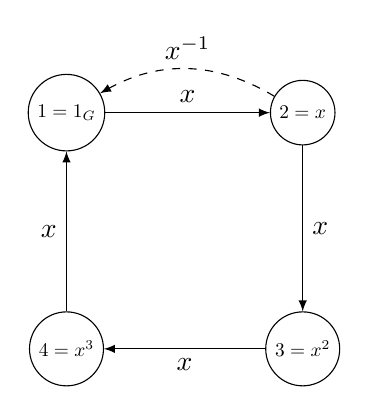
\begin{tikzpicture}
          \node[draw, circle, scale = 0.7] (1) at (0,0) {$1 = 1_G$};
          \node[draw, circle, scale = 0.7] (2) at (3,0) {$2 = x$};
          \node[draw, circle, scale = 0.7] (3) at (3,-3) {$3 = x^2$};
          \node[draw, circle, scale = 0.7] (4) at (0,-3) {$4 = x^3$};
          \draw[->, >=latex] (1) to node[midway, above]{$x$} (2);
          \draw[->, >=latex, dashed] (2) to[bend right] node[midway, above]{$x^{-1}$} (1);
          \draw[->, >=latex] (2) to node[midway, right]{$x$} (3);
          \draw[->, >=latex] (3) to node[midway, below]{$x$} (4);
          \draw[->, >=latex] (4) to node[midway, left]{$x$} (1);
        \end{tikzpicture}
      \end{center}

    \item Soit $G = \langle a, b | a^3 = 1, b^2 = 1, ab = ba^{-1} \iff abab^{-1} = 1 \iff abab = 1
      \rangle$. C'est en fait $Sym(3)$.
      \begin{center}
        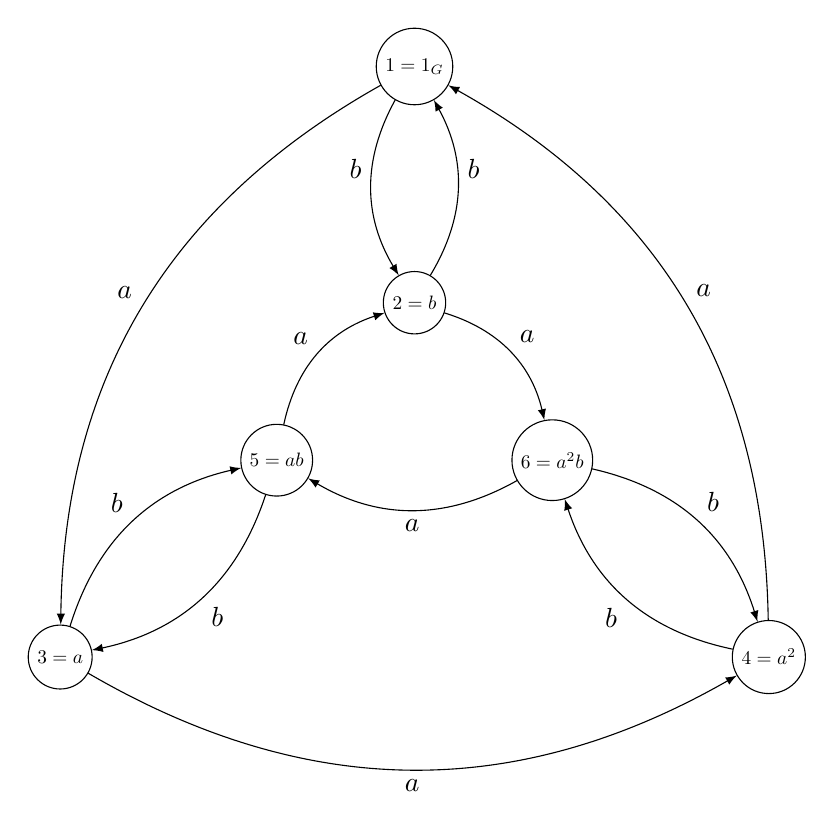
\begin{tikzpicture}
          \node[draw, circle, scale = 0.7] (1) at (0,0) {$1 = 1_G$};
          \node[draw, circle, scale = 0.7] (2) at (0,-3) {$2 = b$};
          \node[draw, circle, scale = 0.7] (3) at (-4.5,-7.5) {$3 = a$};
          \node[draw, circle, scale = 0.7] (4) at (4.5,-7.5) {$4 = a^2$};
          \node[draw, circle, scale = 0.7] (5) at (-1.75,-5) {$5 = ab$};
          \node[draw, circle, scale = 0.7] (6) at (1.75,-5) {$6 = a^2b$};
          \draw[->, >=latex] (1) to[bend right] node[midway, above left]{$a$} (3);
          \draw[->, >=latex] (3) to[bend right] node[midway, below]{$a$} (4);
          \draw[->, >=latex] (4) to[bend right] node[midway, above right]{$a$} (1);
          \draw[->, >=latex] (1) to[bend right] node[midway, above left]{$b$} (2);
          \draw[->, >=latex] (2) to[bend right] node[midway, above right]{$b$} (1);
          \draw[->, >=latex] (2) to[bend left] node[midway, above right]{$a$} (6);
          \draw[->, >=latex] (6) to[bend left] node[midway, below]{$a$} (5);
          \draw[->, >=latex] (5) to[bend left] node[midway, above left]{$a$} (2);
          \draw[->, >=latex] (5) to[bend left] node[midway, below right]{$b$} (3);
          \draw[->, >=latex] (3) to[bend left] node[midway, above left]{$b$} (5);
          \draw[->, >=latex] (6) to[bend left] node[midway, above right]{$b$} (4);
          \draw[->, >=latex] (4) to[bend left] node[midway, below left]{$b$} (6);
        \end{tikzpicture}
      \end{center}
    \end{enumerate}
  \end{exs}

  
  Pour $|G| < \infty$, l'alogrithme de Todd-Coxeter (pour $H = \{1\}$) nous donne le \emph{graphe de Cayley}
  \index{Graphe!de Cayley} (avec les générateurs dans la présentations).


  \subsection{$H \neq \{1\}$ et $|G:H| < \infty$}

  L'algorithme nous donne le \emph{graphe de Schreier} \index{Graphe!de Schreier} de $H$ dans $G$. Les sommets
  sont les classes de $H$ et les arêtes correspondent à l'action de $G$ sur le quotient $G/H$.

  \begin{ex}
    Soit $G = \langle x, y | x^3 = y^3 = (xy)^2 = 1 \rangle$ et soit $H = \langle x \rangle$.
      \begin{center}
        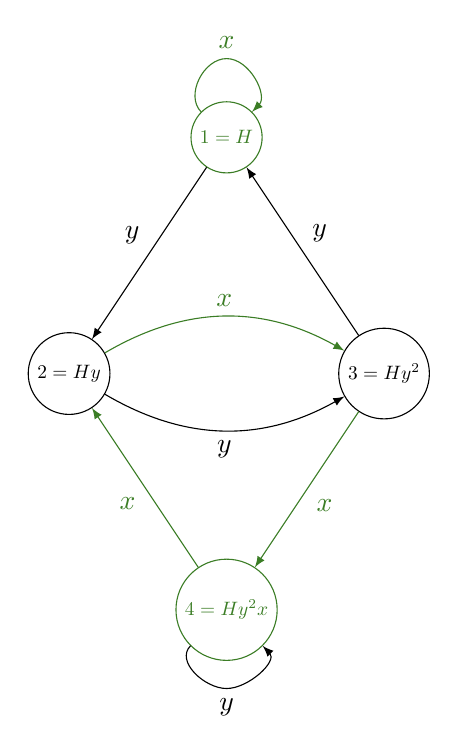
\begin{tikzpicture}
          \node[draw, circle, scale = 0.7, color=OliveGreen] (1) at (0,0) {$1 = H$};
          \node[draw, circle, scale = 0.7] (2) at (-2,-3) {$2 = Hy$};
          \node[draw, circle, scale = 0.7] (3) at (2,-3) {$3 = Hy^2$};
          \node[draw, circle, scale = 0.7, color=OliveGreen] (4) at (0,-6) {$4 = Hy^2x$};
          \draw[->, >=latex, color = OliveGreen] (1.135) to[out=135, in=180] (0, 1) node[above]{$x$}
          to[out=0, in = 45] (1.45);
          \draw[->, >=latex] (1) to node[midway, above left]{$y$} (2);
          \draw[->, >=latex] (3) to node[midway, above right]{$y$} (1);
          \draw[->, >=latex] (2) to[bend right] node[midway, below]{$y$} (3);
          \draw[->, >=latex, color = OliveGreen] (2) to[bend left] node[midway, above]{$x$} (3);
          \draw[->, >=latex, color = OliveGreen] (3) to node[midway, below right]{$x$} (4);
          \draw[->, >=latex] (4.225) to[out=225, in=180] (0, -7) node[below]{$y$} 
          to[out=0, in=315] (4);
          \draw[->, >=latex, color = OliveGreen] (4) to node[midway, below left]{$x$} (2);
        \end{tikzpicture}
      \end{center}
    On a quatres classes, donc l'indice est 4. $H$ n'est pas normal dans $G$, ainsi $G/H$ n'est pas
    nécessairement un groupe, mais juste un ensembles de classes.

    \textbf{Raisonnement pour le graphe:} On cherche ce que vaut $Hxyxy$. Comme $Hx = H$, on en déduit que
    $Hyxy = H$. On doit donc définir $2x = 3$.

    On cherche $Hy^2xy$. Mais $xy = y^{-1}x^{-1}$, ainsi $Hy^2xy = Hyx^2 = 4$.
  \end{ex}




     

%%% Local Variables:
%%% mode: latex
%%% TeX-master: "../GAC_cours.tex" 
%%% End: